\documentclass{article}
\usepackage{graphicx,wrapfig,hyperref,pdfpages,geometry,amsmath,longtable,eurosym,listings,textcomp}

%substitute "{\em PowerEnJoy}" with "\pej"
\newcommand{\pej}{\mbox{\normalfont\itshape PowerEnJoy }}
%substitute "{\em CSGestion}" with "\csg"
\newcommand{\csg}{\mbox{\normalfont\itshape CSGestion }}
\newcommand{\version}{\mbox{\normalfont v. 1.0 }}

%to keep the links of the TOC invisible
\hypersetup{
	colorlinks,
	citecolor=black,
	filecolor=black,
	linkcolor=black,
	urlcolor=black
}

\geometry{margin=1in}



\begin{document}

	%---------------------------	FRONT PAGE      	-----------------------------
	\title{Politecnico di Milano\\A.A. 2016/2017\\Software Engineering 2\\ \bigskip \textbf{C}ode \textbf{I}nspection \version}
	\author{Matteo Bresich (mat. 774366)}
	
	
	%to avoid the hyphenation of the name
	\hyphenation{PowerEnJoy}
	
	\begin{figure}[t]
		\centering
		\includegraphics[width=\linewidth]{"img/logo-polimi"}
		\label{fig:polimi-logo}
	\end{figure}

	\maketitle
	
	%BLANK-PAGE
	\thispagestyle{empty}
	\clearpage\mbox{}\thispagestyle{empty}\clearpage
	
	\renewcommand*\thesection{\arabic{section}}
	\renewcommand*\thesubsection{\arabic{section}.\arabic{subsection}}
	\renewcommand*\thesubsubsection{%
		\arabic{section}.\arabic{subsection}.\arabic{subsubsection}%
	}
	\setcounter{secnumdepth}{4}
	\setcounter{tocdepth}{4}
	
	%---------------------------	TABLE OF CONTENT	-----------------------------
	%to change the page numbering from roman in the toc to arabic
	\pagenumbering{roman}
	\renewcommand{\contentsname}{Table of Content}
	\tableofcontents
	
	\newpage
	\pagenumbering{arabic}
	%to insert the writing "Page" above page numbers in the TOC
	\addtocontents{toc}{~\hfill\textrm{Page}\par}
	
	%---------------------------	INTRODUCTION		-----------------------------
	\section{Classes Assigned}
		The class assigned is part of Apache OFBiz version 16.11.01. \\
		The name of the class assigned is \textit{OfbizAmountTransform.java} and it's located in the following path: \\
		/framework/webapp/src/main/java/org/apache/ofbiz/webapp/ftl/
		
	\section{Functional role of assigned set of classes}
		The OfbizAmountTransform is a class  that implements TemplateTransformModel interface and it is specialized on filtering output.
		The methods analysed are:
		\begin{itemize}
			\item String getArg(Map args, String key) [private static method]
			\item Double getAmount(Map args, String key) [private static method]
			\item Writer getWriter(final Writer out, Map args) [factory method]
			
		\end{itemize}
		\pagebreak
	
	\section{List of issues found by applying the checklist}
		The issues checklist can be found in the document "Code Inspection Assignment Task Description.pdf".
		\subsection{Naming Conventions}
			\begin{enumerate}
				\item \textbf{All class names, interface names, method names, class variables, method variables, and constants used should have meaningful names and do what the name suggests.}
					\begin{itemize}
						\item Class names: no issues.
						\item Interface names: no issues.
						\item Method names: no issues.
						\item Class variables: no issues.
						\item Method variables: no issues, meaningless variable names like "Object o" at line 50, 68 are temporary throwaway variables.
						\item Constants: no issues.
					\end{itemize}
				\item \textbf{If one-character variables are used, they are used only for temporary "throwaway" variables, such as those used in for loops.}
					\begin{itemize}
						\item No issues.
					\end{itemize}
				\item \textbf{Class names are nouns, in mixed case, with the first letter of each word in capitalized.}
					\begin{itemize}
						\item No issues.
					\end{itemize}
				\item \textbf{Interface names should be capitalized like classes.}
					\begin{itemize}
						\item No issues.
					\end{itemize}
				\item \textbf{Method names should be verbs, with the first letter of each addition word capitalized.}
					\begin{itemize}
						\item No issues.
					\end{itemize}
				\item \textbf{Class variables, also called attributes, are mixed case, but might begin with an underscore ('\_') followed by a lowercase first letter. All the remaining words in the variable name have their first letter capitalized.}
					\begin{itemize}
						\item No issues.
					\end{itemize}
				\item \textbf{Constants are declared using all uppercase with words separated by an underscore.}
					\begin{itemize}
						\item issue at line 45 ("module" should be "MODULE").
					\end{itemize}
			\end{enumerate}
			\pagebreak
		\subsection{Indention}
			\begin{enumerate}
				\setcounter{enumi}{7}
				\item \textbf{Three or four spaces are used for indentation and done so consistently.}
					\begin{itemize}
						\item Two spaces instead of four at line 61.
					\end{itemize}
				\item \textbf{No tabs are used to indent.}
					\begin{itemize}
						\item No issues, only spaces used.
					\end{itemize}
			\end{enumerate}
		\subsection{Braces}
			\begin{enumerate}
				\setcounter{enumi}{9}
				\item \textbf{Consistent bracing style is used, either the preferred "Allman" style (first brace goes underneath the opening block) or the "Kernighan and Ritchie" style (first brace is on the same line of the instruction that opens the new block).}
					\begin{itemize}
						\item No issues.
					\end{itemize}
				\item \textbf{All if, while, do-while, try-catch, and for statements that have only one statement to execute are surrounded by curly braces.}
					\begin{itemize}
						\item Issues at lines 52, 69 and 113.
					\end{itemize}
			\end{enumerate}
		\subsection{File Organization}
			\begin{enumerate}
				\setcounter{enumi}{11}
				\item \textbf{Blank lines and optional comments are used to separate sections (beginning comments, package/import statements, class/interface declarations which include class variable/attributes declarations, constructors, and methods).}
				\begin{itemize}
					\item Issues at lines 75, 94 and 98.
				\end{itemize}
				\item \textbf{Where practical, line length does not exceed 80 characters.}
				\begin{itemize}
					\item Issues at lines 18, 52, 69, 95, 113, 120, 128, 129 and 131.
				\end{itemize}
				\item \textbf{When line length must exceed 80 characters, it does NOT exceed 120 characters.}
				\begin{itemize}
					\item No issues.
				\end{itemize}
			\end{enumerate}
		\subsection{Wrapping Lines}
			\begin{enumerate}
				\setcounter{enumi}{14}
				\item \textbf{Line break occurs after a comma or an operator.}
				\begin{itemize}
					\item No issues.
				\end{itemize}
				\item \textbf{Higher-level breaks are used.}
				\begin{itemize}
					\item No issues.
				\end{itemize}
				\item \textbf{A new statement is aligned with the beginning of the expression at the same level as the previous line.}
				\begin{itemize}
					\item No issues.
				\end{itemize}
			\end{enumerate}
		\subsection{Comments}
			\begin{enumerate}
				\setcounter{enumi}{17}
				\item \textbf{Comments are used to adequately explain what the class, interface, methods, and blocks of code are doing.}
				\begin{itemize}
					\item No issues.
				\end{itemize}
				\item \textbf{Commented out code contains a reason for being commented out and a date it can be removed from the source file if determined it is no	longer needed.}
				\begin{itemize}
					\item No issues.
				\end{itemize}
			\end{enumerate}
		\subsection{Java Source Files}
			\begin{enumerate}
				\setcounter{enumi}{19}
				\item \textbf{Each Java source file contains a single public class or interface.}
				\begin{itemize}
					\item No issues.
				\end{itemize}
				\item \textbf{The public class is the first class or interface in the file.}
				\begin{itemize}
					\item No issues.
				\end{itemize}
				\item \textbf{Check that the external program interfaces are implemented consistently with what is described in the javadoc.}
				\begin{itemize}
					\item No issues, TemplateTransformModel interface is implemented consistently.
				\end{itemize}
				\item \textbf{Check that the javadoc is complete (i.e., it covers all classes and files part of the set of classes assigned to you).}
				\begin{itemize}
					\item No issues.
				\end{itemize}
			\end{enumerate}
		\subsection{Package and Import Statements}
			\begin{enumerate}
				\setcounter{enumi}{23}
				\item \textbf{If any package statements are needed, they should be the first non-comment statements. Import statements follow.}
				\begin{itemize}
					\item No issues.
				\end{itemize}
			\end{enumerate}
		\subsection{Class and Interface Declarations}
			\begin{enumerate}
				\setcounter{enumi}{24}
				\item \textbf{The class or interface declarations shall be in order}
				\begin{itemize}
					\item No issues, they are in the correct order.
				\end{itemize}
				\item \textbf{Methods are grouped by functionality rather than by scope or accessibility.}
				\begin{itemize}
					\item No issues.
				\end{itemize}
				\item \textbf{Check that the code is free of duplicates, long methods, big classes,	breaking encapsulation, as well as if coupling and cohesion are adequate.}
				\begin{itemize}
					\item No issues.
				\end{itemize}
			\end{enumerate}
		\subsection{Initialization and Declarations}
			\begin{enumerate}
				\setcounter{enumi}{27}
				\item \textbf{Check that variables and class members are of the correct type. Check	that they have the right visibility (public/private/protected).}
				\begin{itemize}
					\item No issues.
				\end{itemize}
				\item \textbf{Check that variables are declared in the proper scope.}
				\begin{itemize}
					\item No issues.
				\end{itemize}
				\item \textbf{Check that constructors are called when a new object is desired.}
				\begin{itemize}
					\item Some objects are not initialized by the constructor at lines: 45, 46, 49, 50, 68, 77, 81, 85, 95, 96, 97, 114, 117 and 118.
				\end{itemize}
				\item \textbf{Check that all object references are initialized before use.}
				\begin{itemize}
					\item No issues.
				\end{itemize}
				\item \textbf{Variables are initialized where they are declared, unless dependent upon a computation.}
				\begin{itemize}
					\item No issues.
				\end{itemize}
				\item \textbf{Declarations appear at the beginning of blocks (A block is any code surrounded by curly braces '\{' and '\}'). The exception is a variable can be declared in a for loop.}
				\begin{itemize}
					\item Issue at line 114.
				\end{itemize}
			\end{enumerate}
		\subsection{Method Calls}
			\begin{enumerate}
				\setcounter{enumi}{33}
				\item \textbf{Check that parameters are presented in the correct order.}
				\begin{itemize}
					\item No issues.
				\end{itemize}
				\item \textbf{Check that the correct method is being called, or should it be a different method with a similar name.}
				\begin{itemize}
					\item No issues.
				\end{itemize}
				\item \textbf{Check that method returned values are used properly.}
				\begin{itemize}
					\item No issues.
				\end{itemize}
			\end{enumerate}
		\subsection{Arrays}
			\begin{enumerate}
				\setcounter{enumi}{36}
				\item \textbf{Check that there are no off-by-one errors in array indexing (that is, all required array elements are correctly accessed through the index).}
				\begin{itemize}
					\item No issues.
				\end{itemize}
				\item \textbf{Check that all array (or other collection) indexes have been prevented from going out-of-bounds.}
				\begin{itemize}
					\item No issues.
				\end{itemize}
				\item \textbf{Check that constructors are called when a new array item is desired.}
				\begin{itemize}
					\item No issues.
				\end{itemize}
			\end{enumerate}
		\subsection{Object Comparison}
			\begin{enumerate}
				\setcounter{enumi}{39}
				\item \textbf{Check that all objects (including Strings) are compared with equals and not with ==.}
				\begin{itemize}
					\item No issues. (At line 72 the == is not a comparison and it is used to check that the variable o is null).
				\end{itemize}
			\end{enumerate}
		\subsection{Output Format}
			\begin{enumerate}
				\setcounter{enumi}{40}
				\item \textbf{Check that displayed output is free of spelling and grammatical errors.}
				\begin{itemize}
					\item No issues.
				\end{itemize}
				\item \textbf{Check that error messages are comprehensive and provide guidance as to how to correct the problem.}
				\begin{itemize}
					\item No issues.
				\end{itemize}
				\item \textbf{Check that the output is formatted correctly in terms of line stepping and spacing.}
				\begin{itemize}
					\item No issues.
				\end{itemize}
			\end{enumerate}
		\subsection{Computation, Comparisons and Assignments}
			\begin{enumerate}
				\setcounter{enumi}{43}
				\item \textbf{Check that the implementation avoids "brutish programming"}
				\begin{itemize}
					\item No issues.
				\end{itemize}
				\item \textbf{Check order of computation/evaluation, operator precedence and parenthesizing.}
				\begin{itemize}
					\item No issues.
				\end{itemize}
				\item \textbf{Check the liberal use of parenthesis is used to avoid operator precedence problems.}
				\begin{itemize}
					\item No issues.
				\end{itemize}
				\item \textbf{Check that all denominators of a division are prevented from being zero.}
				\begin{itemize}
					\item No issues.
				\end{itemize}
				\item \textbf{Check that integer arithmetic, especially division, are used appropriately to avoid causing unexpected truncation/rounding.}
				\begin{itemize}
					\item No issues.
				\end{itemize}
				\item \textbf{Check that the comparison and Boolean operators are correct.}
				\begin{itemize}
					\item No issues.
				\end{itemize}
				\item \textbf{Check throw-catch expressions, and check that the error condition is actually legitimate.}
				\begin{itemize}
					\item No issues.
				\end{itemize}
				\item \textbf{Check that the code is free of any implicit type conversions.}
				\begin{itemize}
					\item No issues.
				\end{itemize}
			\end{enumerate}
		\subsection{Exceptions}
			\begin{enumerate}
				\setcounter{enumi}{51}
				\item \textbf{Check that the relevant exceptions are caught.}
				\begin{itemize}
					\item No issues.
				\end{itemize}
				\item \textbf{Check that the appropriate action are taken for each catch block.}
				\begin{itemize}
					\item No issues.
				\end{itemize}
			\end{enumerate}
		\subsection{Flow of Control}
			\begin{enumerate}
				\setcounter{enumi}{53}
				\item \textbf{In a switch statement, check that all cases are addressed by break or
					return.}
				\begin{itemize}
					\item No issues.
				\end{itemize}
				\item \textbf{Check that all switch statements have a default branch.}
				\begin{itemize}
					\item No issues.
				\end{itemize}
				\item \textbf{Check that all loops are correctly formed, with the appropriate initialization, increment and termination expressions.}
				\begin{itemize}
					\item No issues.
				\end{itemize}
			\end{enumerate}
		\subsection{Files}
			\begin{enumerate}
				\setcounter{enumi}{56}
				\item \textbf{Check that all files are properly declared and opened.}
				\begin{itemize}
					\item No issues.
				\end{itemize}
				\item \textbf{Check that all files are closed properly, even in the case of an error.}
				\begin{itemize}
					\item No issues.
				\end{itemize}
				\item \textbf{Check that EOF conditions are detected and handled correctly.}
				\begin{itemize}
					\item No issues.
				\end{itemize}
				\item \textbf{Check that all file exceptions are caught and dealt with accordingly.}
				\begin{itemize}
					\item No issues.
				\end{itemize}
			\end{enumerate}
		\pagebreak
	\section{Other Issues}
		In the class additional problems were found:
		\begin{itemize}
			\item line 49: the space is doubled
			\item lines 52, 69, 113: two statements per line instead of one \\
			
			\begin{minipage}{\linewidth}
				\vspace{2mm}
				\makebox[\linewidth]{
					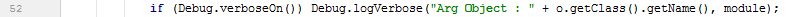
\includegraphics[keepaspectratio=true,scale=0.5]{img/other_issue_52}}
				\vspace{2mm}
			\end{minipage}
			\item line 99: the anonymous class should be better if it was a named class (too complex for an anonymous class). \\
			
			\begin{minipage}{\linewidth}
				\vspace{2mm}
				\makebox[\linewidth]{
					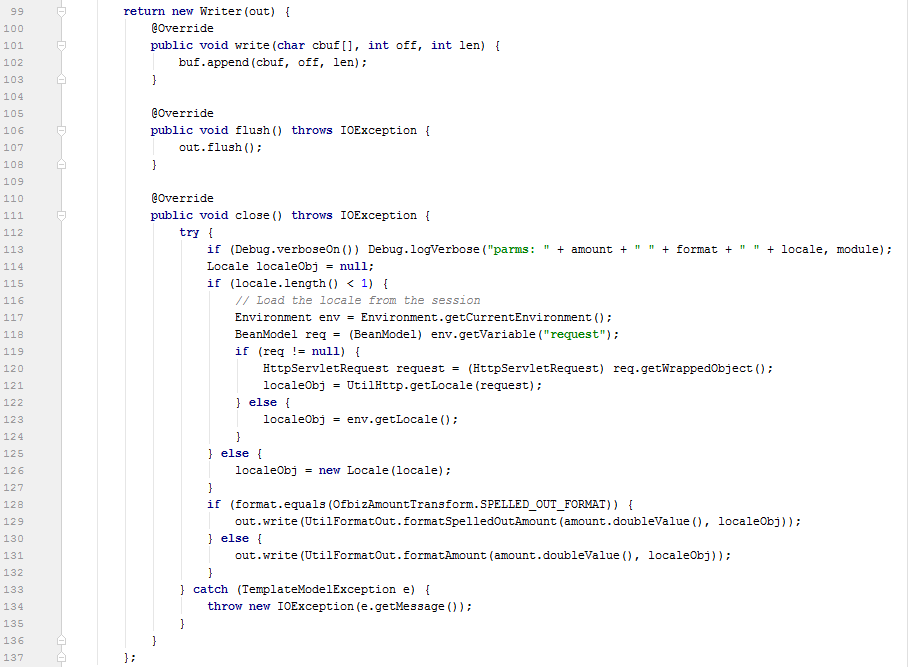
\includegraphics[keepaspectratio=true,scale=0.6]{img/other_issue_99}}
				\vspace{2mm}
			\end{minipage}
			\item line 114: useless assignment \\
			
			\begin{minipage}{\linewidth}
				\vspace{2mm}
				\makebox[\linewidth]{
					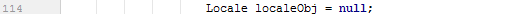
\includegraphics[keepaspectratio=true,scale=0.6]{img/other_issue_114}}
				\vspace{2mm}
			\end{minipage}
		\end{itemize}
		\pagebreak
	\section{Effort Spent}
		\subsection{Hours of work} The time spent to redact this document:
		\begin{itemize}
			\item Bresich Matteo: 16 hours.
		\end{itemize}
		
		\begin{center}
			\begin{tabular}{ | l | l |}
				\hline
				Days & Hours of work\\ \hline
				01/02/17 & 4h\\\hline
				02/01/17 & 4h\\\hline
				04/01/17 & 4h\\\hline
				05/01/17 & 4h\\\hline
			\end{tabular}
		\end{center}
	\section{References}
		\begin{itemize}
			\item TeXstudio v2.11.2 (http://www.texstudio.org/) to produce this document.
			\item IntelliJ IDEA ULTIMATE 2016.3.2 (https://www.jetbrains.com/idea/) to inspect the assigned class.
			\item SonarLint v2.7.1.1640 (IntelliJ plug-in): plugin for code analysis.
			\item Sublime Text 3: to inspect the assigned class.
		\end{itemize}
	
\end{document}